
\documentclass[11pt,titlepage,a4paper]{report}

%INCLUSIONE PACCHETTI
%---------------------------------------------
\usepackage[italian]{babel}
\usepackage{fancyhdr}
\usepackage{graphicx}
\graphicspath{{./pics/}} % cartella di salvataggio immagini

% STILE DI PAGINA
%---------------------------------------------
\pagestyle{fancy}
\renewcommand{\sectionmark}[1]{\markright{\thesection.\ #1}}
\lhead{\nouppercase{\rightmark}}
\rhead{\nouppercase{\leftmark}}
\renewcommand{\chaptermark}[1]{%
\markboth{\thechapter.\ #1}{}}

%Ridefinisco lo stile plain della pagina
\fancypagestyle{plain}{%
	\lhead{
\includegraphics[height=50pt]{logo.eps}}
	\chead{}
	\rhead{HappyCode inc \\ happycodeinc@gmail.com}
	\lfoot{BR-jsys}
	\cfoot{\thepage}
	\renewcommand{\headrulewidth}{1pt}
	\renewcommand{\footrulewidth}{1pt}
}
% layout
\begin{document}
%definizione variabili 
\newcommand{\lv}{2.8} % latest version
\newcommand{\dt}{ Analisi Dei Requisiti }% Document title
%common variables
\newcommand{\br}{\underline{business rule}}
\newcommand{\brs}{\underline{business rules}}
\newcommand{\bo}{\underline{business object}}
\newcommand{\bos}{\underline{business objects}}
\newcommand{\rp}{\underline{repository}}
\newcommand{\brp}{BusinessRuleParser}
\newcommand{\brl}{BusinessRuleLexer}
\newcommand{\BR}{\underline{BusinessRule}}

%nomi dei componenti
\newcommand{\AT}{Alessia Trivellato}
\newcommand{\ET}{Elena Trivellato}
\newcommand{\FC}{Filippo Carraro}
\newcommand{\LA}{Luca Appon}
\newcommand{\MB}{Michele Bortolato}
\newcommand{\MT}{Marco Tessarotto}
\newcommand{\MM}{Mattia Meroi}%altre variabili
% ultime versioni dei documenti da modificare solo alla fine
\newcommand{\AR}{AnalisiDeiRequisiti.2.6.pdf}
\newcommand{\DdP}{DefinizioneDiProdotto.0.9.pdf}
\newcommand{\G}{ Glossario.1.8.pdf }
\newcommand{\NdP}{NormeDiProgetto.2.0.pdf}
\newcommand{\PdQ}{ PianoDiQualifica.2.0.pdf }
\newcommand{\PdP}{ PianoDiProgetto.1.7.pdf }
\newcommand{\ST}{SpecificaTecnica.1.5.pdf}
\newcommand{\TR}{TestReport.0.7.pdf}
\newcommand{\MU}{ManualeUtente.0.3.pdf}%nomi documenti
%fine definizione variabili
\hyphenation{
 a-na-lo-go
 as-so-cia-zio-ne
 %attività non si può inserire come tutte le parole accentate che vanno messe nel testo semplice scritte at\-ti\-vi\-tà o come variabile
 coe-ren-za
 com-po-nen-ti
 des-crit-te
 des-cri-zio-ni
 di-a-gram-ma
 di-a-gram-mi
 e-le-men-to
 e-se-gui-re
 e-si-sten-ti
 es-pli-ci-to
 glo-bal-men-te
 glos-sa-rio
 li-vel-lo
 ne-ces-sa-rio
 per-met-te-re
 re-po-si-to-ry
 re-vi-sio-na-men-to
 ri-chies-te
 se-gna-la-ta
 va-li-da-zio-ne
 va-ria-bi-li
 ve-ri-fi-ca-re
 vi-sua-liz-za-te
 e-ven-tua-li
 o-pe-ra-zio-ne
 ar-chi-via-zio-ne
 mo-di-fi-ca
}


%sillabazione
\begin{titlepage}
\begin{center}
\vspace*{0.5in}

\includegraphics{logo.eps}
\vspace*{0.2in}

{\Large \textbf{BR-jsys}}
{\Large \emph{business rules} per sistemi gestionali in architettura J2EE } 
\vspace{2in}

\Huge \textsc{ \dt }

\end{center}
\end{titlepage}
\vspace*{0.5in}%pagina del titolo


\begin{center}
\thispagestyle{plain}
\begin{table}[htbp]
\large{
\begin{tabular}{l}
\Large{\textbf{\textsf{Capitolato: ''\underline{BR-jsys}``}}} \\
\begin{tabular}{|p{6cm}|p{6cm}|} \hline
\textbf{Data creazione:} & 18/11/2007 \\ \hline
\textbf{Versione:} & \lv \\ \hline
\textbf{Stato del documento:} & formale, esterno \\ \hline
% ----------------------------------------------------------------------------autori
\textbf{Revisione RR} &   \\ \hline
\textbf{Redazione:} & \MB, \AT \\ \hline
\textbf{Revisione:} &   \MT \\ \hline
\textbf{Approvazione:}  & \ET \\ \hline
\textbf{Revisione RPD} &  \\ \hline 
\textbf{Redazione:} & \MT \\ \hline
\textbf{Revisione:} &  \AT, \MB \\ \hline
\textbf{Approvazione:}  & \ET \\ \hline
\textbf{Revisione RQ} &   \\ \hline
\textbf{Redazione:} & \ET \\ \hline
\textbf{Revisione:} & \\ \hline
\textbf{Approvazione:}  & \\ \hline
%------------------------------------------------------------------------------

\end{tabular} \\
\end{tabular}
}
\end{table}

\begin{table}[hbtp]
\large{
\begin{tabular}{l}
\Large{\textbf{\textsf{Lista di distribuzione}}} \\
\begin{tabular}{|p{6cm}|p{6cm}|} \hline
%  -------------------------------------------------------------lista di distribuzione
{HappyCode inc}& Gruppo di lavoro\\ \hline
{Tullio Vardanega, Renato Conte}& Committenti \\ \hline 
{Zucchetti S.r.l}& Azienda proponente\\ \hline
\end{tabular} \\
\end{tabular}
}
\end{table}
\begin{table}[hbtp]

\Large{\textbf{\textsf{Diario delle modifiche}}} \\
\begin{small}
\begin{tabular}[t]{|p{1,2cm}|p{1.9cm}|p{2.9cm}|p{5cm}|} \hline
Versione & Data & Autore & Descrizione \\ \hline
%-------------------------------------------------------------------------------diario modifiche
3.1 & 05/03/2208 & \MM & Eliminazione sezione ''Descrizione del resto del documento`` perch\'e inutile.\\ \hline
3.0 & 05/03/2008 & \MM & Evidenziazione dei termini contenuti nel documento \G .\\ \hline
2.9 & 04/03/2008 & \MM & Aggiunta di link ipertestuali all'indice del documento.\\ \hline
2.8 & 04/03/2008 & \MT & Modifica al layout, introduzione totale pagine e autori nel diario delle modifiche.\\ \hline
2.7 & 03/03/2008 & \ET & Aggiunta tabella di tracciamento dei requisiti\\ \hline 
2.6 & 14/02/2008 & \MB & Correzione sintattica e grammaticale\\ \hline
2.5 & 11/02/2008 & \LA & Deprecato requisito F9 e modificato i requisiti F4 e F8\\ \hline
2.4 & 05/02/2008 & \MT & Aggiunta del nome del file nel modello di documento\\ \hline
2.3 & 04/02/2008 & \AT & Correzione grammaticale\\ \hline
2.2 & 22/01/2008 & \MT & Modifica al layout dei documenti e prima correzione grammaticale\\ \hline
2.1 & 21/01/2008 & \MM & Modifiche in conseguenza del secondo incontro con l'azienda\\ \hline
2.0 & 10/01/2008 & \MT & Inserito tracciamento dei requisiti\\ \hline
1.4 & 09/01/2008 & \MT & Modifiche alla struttura del documento e all'ordine dei paragrafi\\ \hline
1.3 & 03/01/2008 & \MB & Modifiche ai casi d'uso e alla loro analisi\\ \hline
1.2 & 21/12/2007 & \MT & Documento sottoposto a revisionamento automatico\\ \hline
1.1 & 03/12/2007 & \MT & Correzioni grammaticali, correzioni strutturali\\ \hline
1.0 & 28/11/2007 & \MB & Inserimento casi d'uso\\ \hline
0.2 & 22/11/2007 & \MB & Aggiornamento requisiti \\ \hline
0.1 & 18/11/2007 & \AT & Stesura preliminare del documento \\ \hline

\end{tabular} \\
\end{small}


\end{table}
\end{center}
\newpage

\tableofcontents

\chapter{Introduzione}
\section{Scopo del documento}
Il presente documento viene redatto al fine di identificare i requisiti presenti nel capitolato d'appalto denominato \underline{BR-jsys}, conseguire il raggiungimento dell'obiettivo richiesto e soddisfare le esigenze di tutti gli stakeholders coinvolti nella realizzazione del progetto di cui sopra.
\section{Scopo del prodotto}
Il prodotto andr\`a inserito in un progetto pi\`u ampio. Il suo obiettivo \`e quello di testare la consistenza di business objects, altrimenti difficilmente verificabile tramite vincoli relazionali.
Verr\`a creato quindi un linguaggio per la definizione di \\underline{Business Rules}. Quest'ultime verranno immagazzinate in un \textit{file repository}; nel momento in cui l'utente avr\`a bisogno di verificare la consistenza di un business object, un interprete si preoccuper\`a di invocare ed eseguire le regole che lo riguardano, stabilendo cos\`i se esso le rispetta tutte o meno.
Il progetto dovr\`a integrarsi infine con le componenti gi\`a sviluppate dall'azienda proponente. In particolare dovr\`a interfacciarsi con il loro interprete, il quale dovr\`a poi applicare le regole ai business objects.
\section{Definizioni, acronimi, abbreviazioni}
Nella tabella di seguito vengono riportate tutte le abbreviazioni utlizzate nel documento, comprese le sigle utilizzate per il tracciamento dei requisiti.
\begin{center}
\begin{tabular}{||p{3.0cm}||p{8.5cm}||} \hline
\textbf{Abbreviazione} & \textbf{Significato} \\ \hline
C04 & Indica il quarto capitolato d'appalto denominato \underline{BR-jsys}.\\ \hline
I01 & Indica il primo incontro avuto con il proponente descritto nel documento Incontro2007-11-22.pdf\\ \hline
I02 & Indica il secondo incontro avuto con il proponente descritto nel documento Incontro2008-01-17.pdf\\ \hline
F\textit{\#} & Con F seguito da un numero intero sono indicati i requisiti funzionali.\\ \hline
NU\textit{\#} & Con NU seguito da un numero intero sono indicati i requisiti di usabilit\`a.\\ \hline
NPo\textit{\#} & Con NPo seguito da un numero intero sono indicati i requisiti di portabilit\`a.\\ \hline
NPr\textit{\#} & Con Npr seguito da un numero intero sono indicati i requisiti prestazionali.\\ \hline
NQ\textit{\#} & Con NQ seguito da un numero intero sono indicati i requisiti di qualit\`a.\\ \hline

\end{tabular} \\
\end{center}
\subsection{Glossario}
Per gli altri termini non citati nella tabella soprastante si fa riferimento al file esterno \G. I termini che sono presenti nel \G sono sottolineati.
\section{Riferimenti}
\begin{itemize}
\item Capitolato d'appalto concorso per sistema ``\underline{BR-jsys}'';
\item Verbale dell'incontro con il proponente ``Incontro2007-11-22.pdf'';
\item Verbale dell'incontro con il proponente ``Incontro2008-02-05.pdf'';
\item ``Ingegneria del Software'' 8a edizione - Ian Sommerville.
\end{itemize}
%----------------------------------------------------------------------------------inserire il libro 
\chapter{Descrizione generale}
\section{Prospettiva del prodotto}
Il sistema va a collocarsi all'interno di un progetto globale di automazione nella generazione del codice per la produzione di software gestionale. In particolare si occuper\`a della gestione delle \\underline{Business Rules}, definendo un linguaggio con cui descriverle, oltre ad un sistema di archiviazione-recupero delle stesse.
\section{Funzioni del prodotto}
Il sistema si occupa di definire un linguaggio con cui descrivere \\underline{Business Rules}. Pi\`u concretamente dovr\`a verificare che le \\underline{Business Rules} inserite dall'utente rispettino il linguaggio sopra citato. In caso di esito positivo dovranno essere inserite in un repository, dal quale potranno poi essere recuperate nel momento in cui si desideri verificare la consistenza di un business object.
\section{Caratteristiche utente}
Il sistema andr\`a inserito all'interno di un progetto pi\`u ampio, il cui utente finale \`e un individuo esperto in ambito commerciale e gestionale, ma non necessariamente in ambito informatico.
\section{Vincoli generali}
Il linguaggio di programmazione adottato per lo sviluppo del prodotto sar\`a Java. Il sistema dovr\`a inoltre potersi interfacciare con le componenti gi\`a sviluppate dall'azienda proponente. 
\section{Presupposti e dipendenze}
\begin{itemize}
\item{Le \\underline{Business Rules} su cui si opera saranno di tipo \textit{\underline{Rejector}}. Una \underline{Business Rule} deve essere composta da uno o pi\`u confronti tra espressioni dello stesso tipo (eventualmente complesse).}
\item{I business objects che manipoleremo sono generalmente costituiti da campi dati semplici (numeri reali, booleani, stringhe), da un insieme di array o vettori omogenei tutti della stessa lunghezza (derivanti da tabelle) e da riferimenti ad altri business objects (ma non da array di business objects).
}
\item{La virtual machine utilizzata  per sviluppare gli oggetti richiesti \`e Java 1.6.}
\end{itemize}

\chapter{Requisiti Specifici}
Per illustrare e rendere pi\`u chiaro il sistema e le sue componenti, verranno qui presi in considerazione dei diagrammi use-case \underline{UML}. Verranno elencati in seguito i requisiti individuati, ognuno dei quali preceduto da una sigla identificativa e seguito da una sigla che indica il documento da cui proviene.


\section{Inserimento e cancellazione di \underline{Business Rule}.}
\begin{center}
 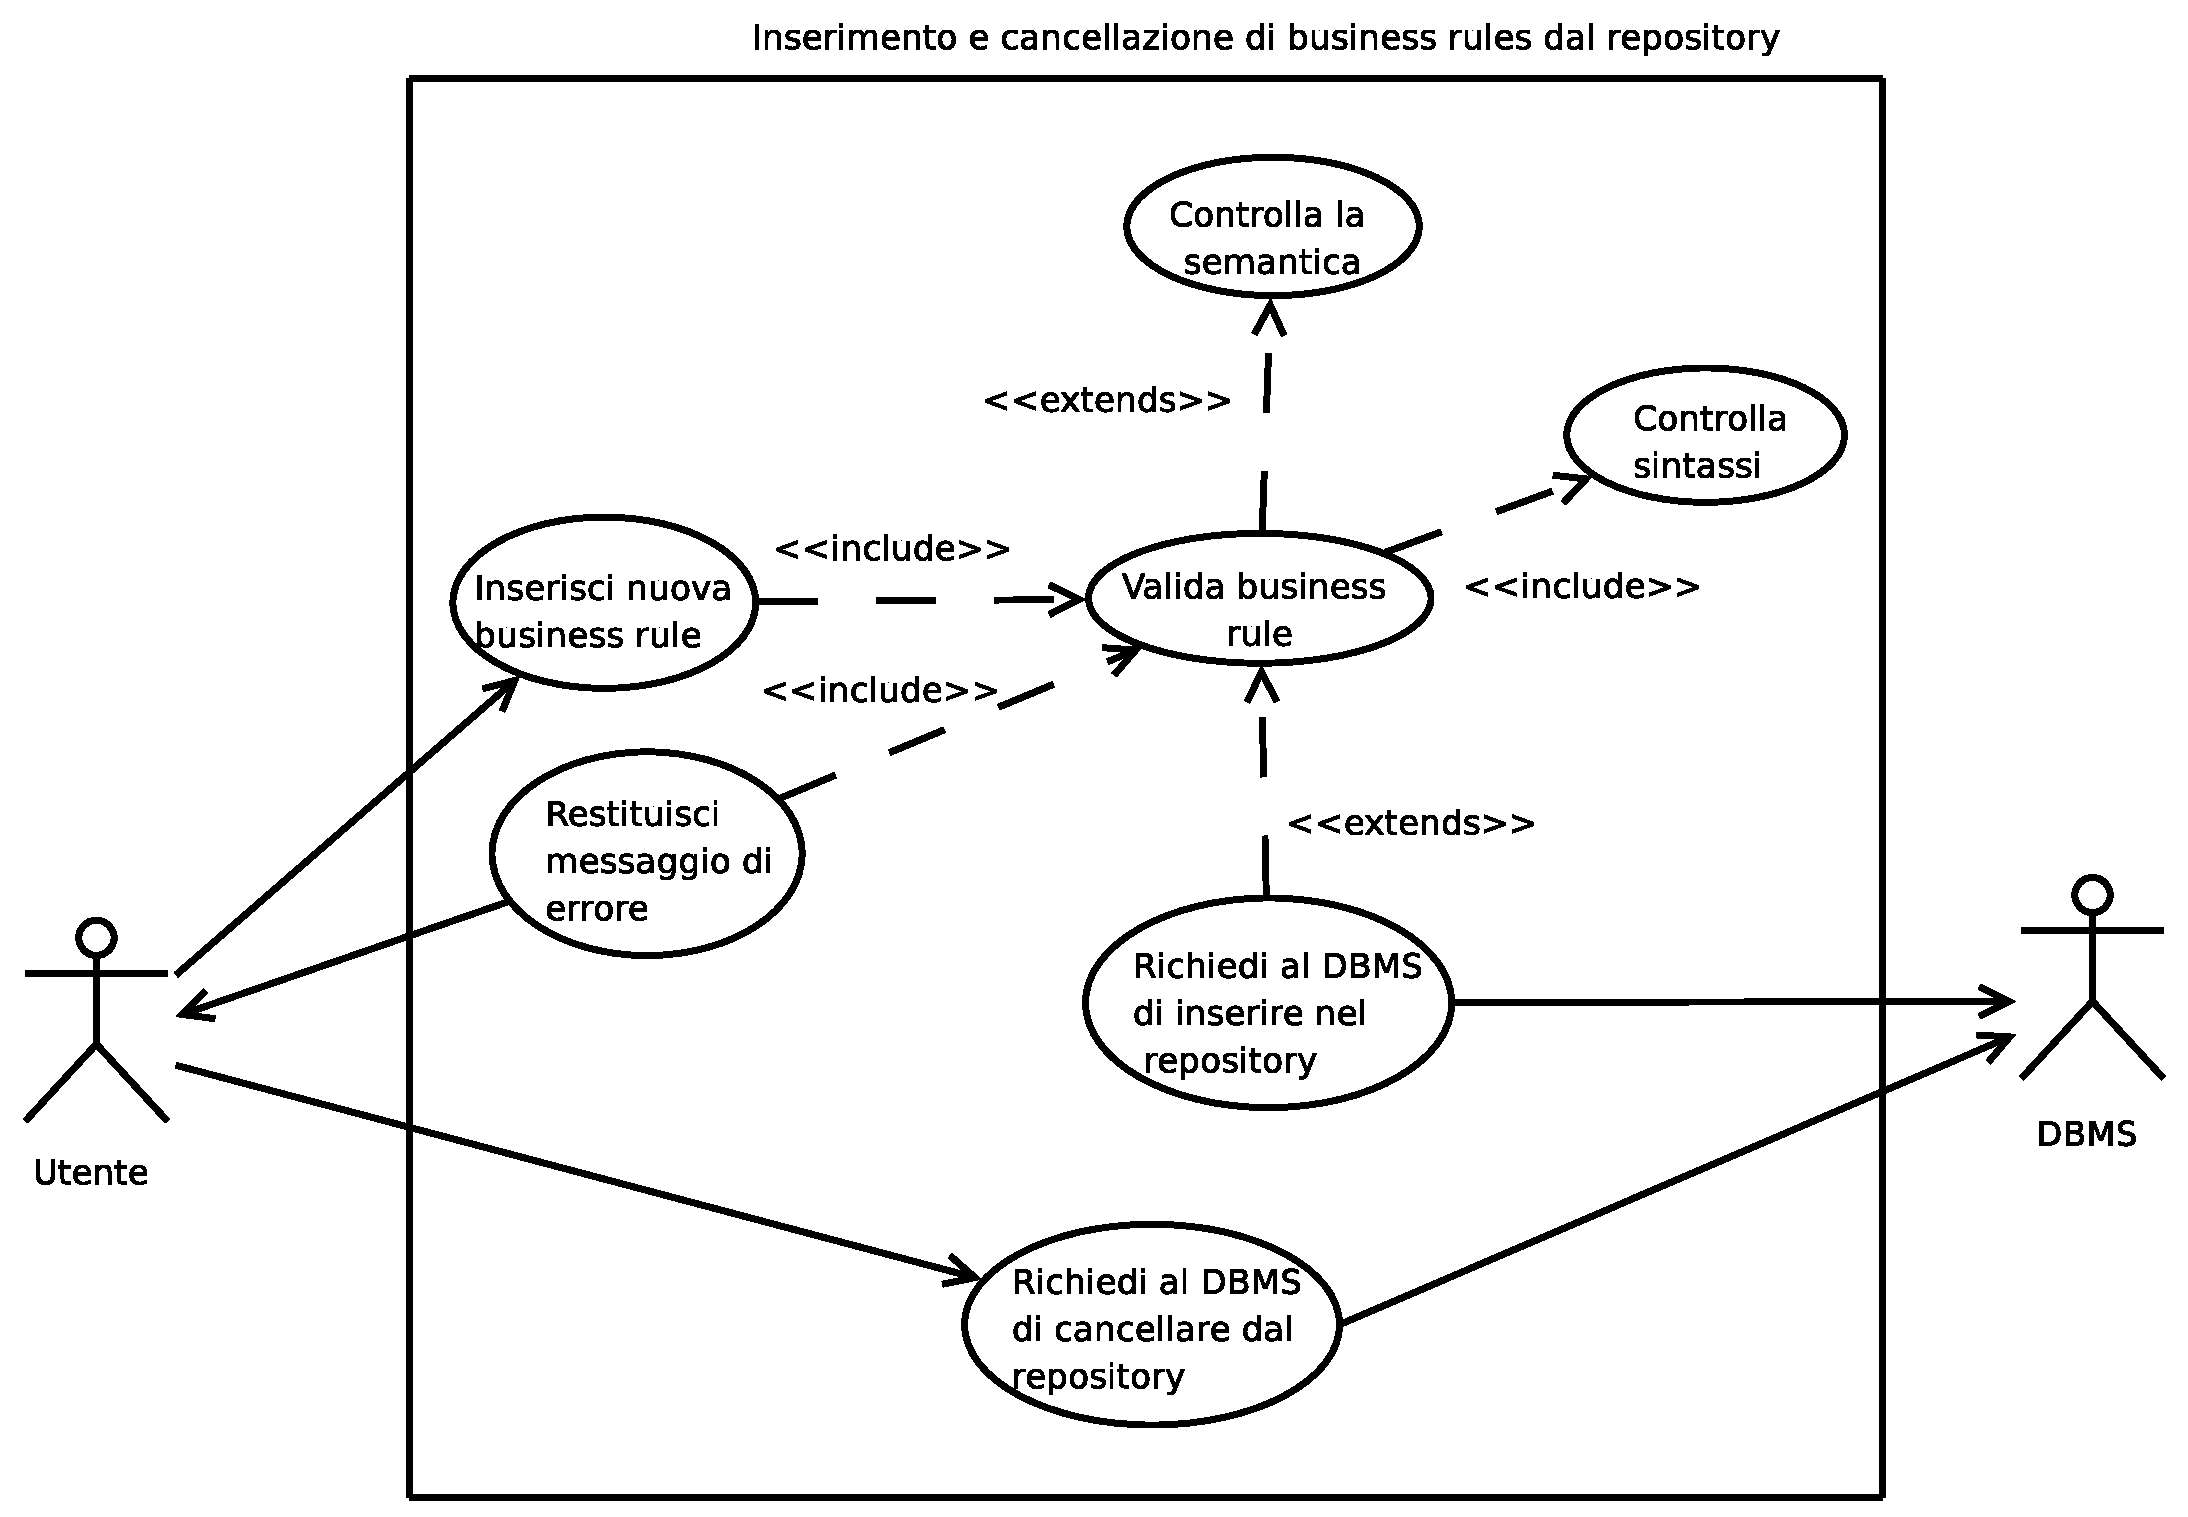
\includegraphics[width=1\textwidth]{use-case/Inserisci-regola.eps}
\end{center}

\subsection{Inserisci nuova \underline{Business Rule}.}
\textbf{Attori coinvolti:} L'utente finale che desidera inserire nel repository una nuova \underline{Business Rule}.\\
\textbf{Scopo e descrizione sintetica:} Il sistema riceve in ingresso una nuova \underline{Business Rule} che dovr\`a essere validata.\\
\textbf{Flusso di eventi:} Il sistema acquisisce la nuova \underline{Business Rule} appena inserita dall'utente e la invia successivamente al validatore.\\
\textbf{Precondizioni:} L'utente ha inserito una nuova \underline{Business Rule}.\\
\textbf{Postcondizioni} La \underline{Business Rule} viene inviata al validatore.

\subsection{Valida \underline{Business Rule}.}
\textbf{Scopo e descrizione sintetica:} Il validatore riceve in ingresso la \underline{Business Rule} e si preoccupa di eseguire una serie di controlli per la sua validazione.\\
\textbf{Flusso di eventi:} Il validatore una volta acquisita la \underline{Business Rule} la sottopone a diversi controlli per poterla validare.\\
\textbf{Precondizioni:} Il sistema ha acquisito una nuova \underline{Business Rule}.\\
\textbf{Postcondizioni} La \underline{Business Rule} viene inviata alla componente che valida la sintassi.
 
\subsection{Controlla sintassi.}
\textbf{Scopo e descrizione sintetica:} Si controlla che la nuova \underline{Business Rule} sia formulata secondo le specifiche e la sintassi del linguaggio scelto.\\
\textbf{Flusso di eventi:} Viene controllata la sintassi della nuova \underline{Business Rule} appena inserita.\\
\textbf{Precondizioni:} Il validatore ha inviato la \underline{Business Rule} al controllo della sintassi.\\
\textbf{Postcondizioni} La \underline{Business Rule} pu\`o avanzare al successivo controllo.

\subsection{Controlla la semantica.}
\textbf{Scopo e descrizione sintetica:} Si controllano i tipi nella nuova \underline{Business Rule} e si verifica che i campi dati utilizzati siano realmente presenti nel business object associato.\\
\textbf{Flusso di eventi:} Vengono controllati i tipi nella \underline{Business Rule} e la corrispondenza tra i campi dati usati nella \textbf{Business Rule} e quelli presenti nel business object ad essa associato.\\
\textbf{Precondizioni:} Il validatore ha inviato la \underline{Business Rule} al controllo semantico.\\
\textbf{Postcondizioni} La \underline{Business Rule} \`e pronta per essere inserita nel \textit{repository}.

\subsection{Restituisci messaggio di errore.}
\textbf{Attori coinvolti:} L'utente finale che ha cercato di inserire una nuova \underline{Business Rule} e non ci \`e riuscito.\\
\textbf{Scopo e descrizione sintetica:} Il sistema comunica all'utente che la \underline{Business Rule} inserita presenta degli errori.\\
\textbf{Flusso di eventi:} Il sistema  a fronte di un errore nella validazione della \underline{Business Rule} invia una segnalazione dell'errore all'utente.\\
\textbf{Precondizioni:} La validazione non \`e andata a buon fine.\\
\textbf{Postcondizioni} L'utente riceve un messaggio che lo informa dell'errore commesso nella creazione della nuova \underline{Business Rule}.

\subsection{Richiedi al \underline{DBMS} di inserire nel repository.}
\textbf{Attori coinvolti:} Il \underline{DBMS} che si preoccuper\`a di inserire la regola nel repository.\\
\textbf{Scopo e descrizione sintetica:} Il sistema comunica al \underline{DBMS} che la \underline{Business Rule} \`e stata validata e pu\`o essere inserita nel repository.\\
\textbf{Flusso di eventi:} Il sistema  terminata la validazione invia la \underline{Business Rule} al \underline{DBMS} che si preoccuper\`a di inserirla nel \textit{repository}.\\
\textbf{Precondizioni:} La validazione \`e terminata senza errori.\\
\textbf{Postcondizioni} Il \underline{DBMS} inserir\`a la \underline{Business Rule} nel \textit{repository}.

\subsection{Richiedi al \underline{DBMS} di cancellare dal repository.}
\textbf{Attori coinvolti:} L'utente finale che richiede al sistema di cancellare una \underline{Business Rule} dal repository e il \underline{DBMS} che si preoccuper\`a di cancellarla.\\
\textbf{Scopo e descrizione sintetica:} Il sistema mette in comunicazione l'utente finale col \underline{DBMS} richiedendo al \underline{DBMS} la cancellazione della \underline{Business Rule} indicata dall'utente\\
\textbf{Flusso di eventi:} Il sistema riceve la richiesta di cancellazione di una \underline{Business Rule} e la comunica al \underline{DBMS}.\\
\textbf{Precondizioni:} L'utente ha chiesto che una determinata \underline{Business Rule} venga cancellata.\\
\textbf{Postcondizioni} Il \underline{DBMS} canceller\`a la \underline{Business Rule} dal \textit{repository}.


\section{Recupera \\underline{Business Rules}.}
\begin{center}
 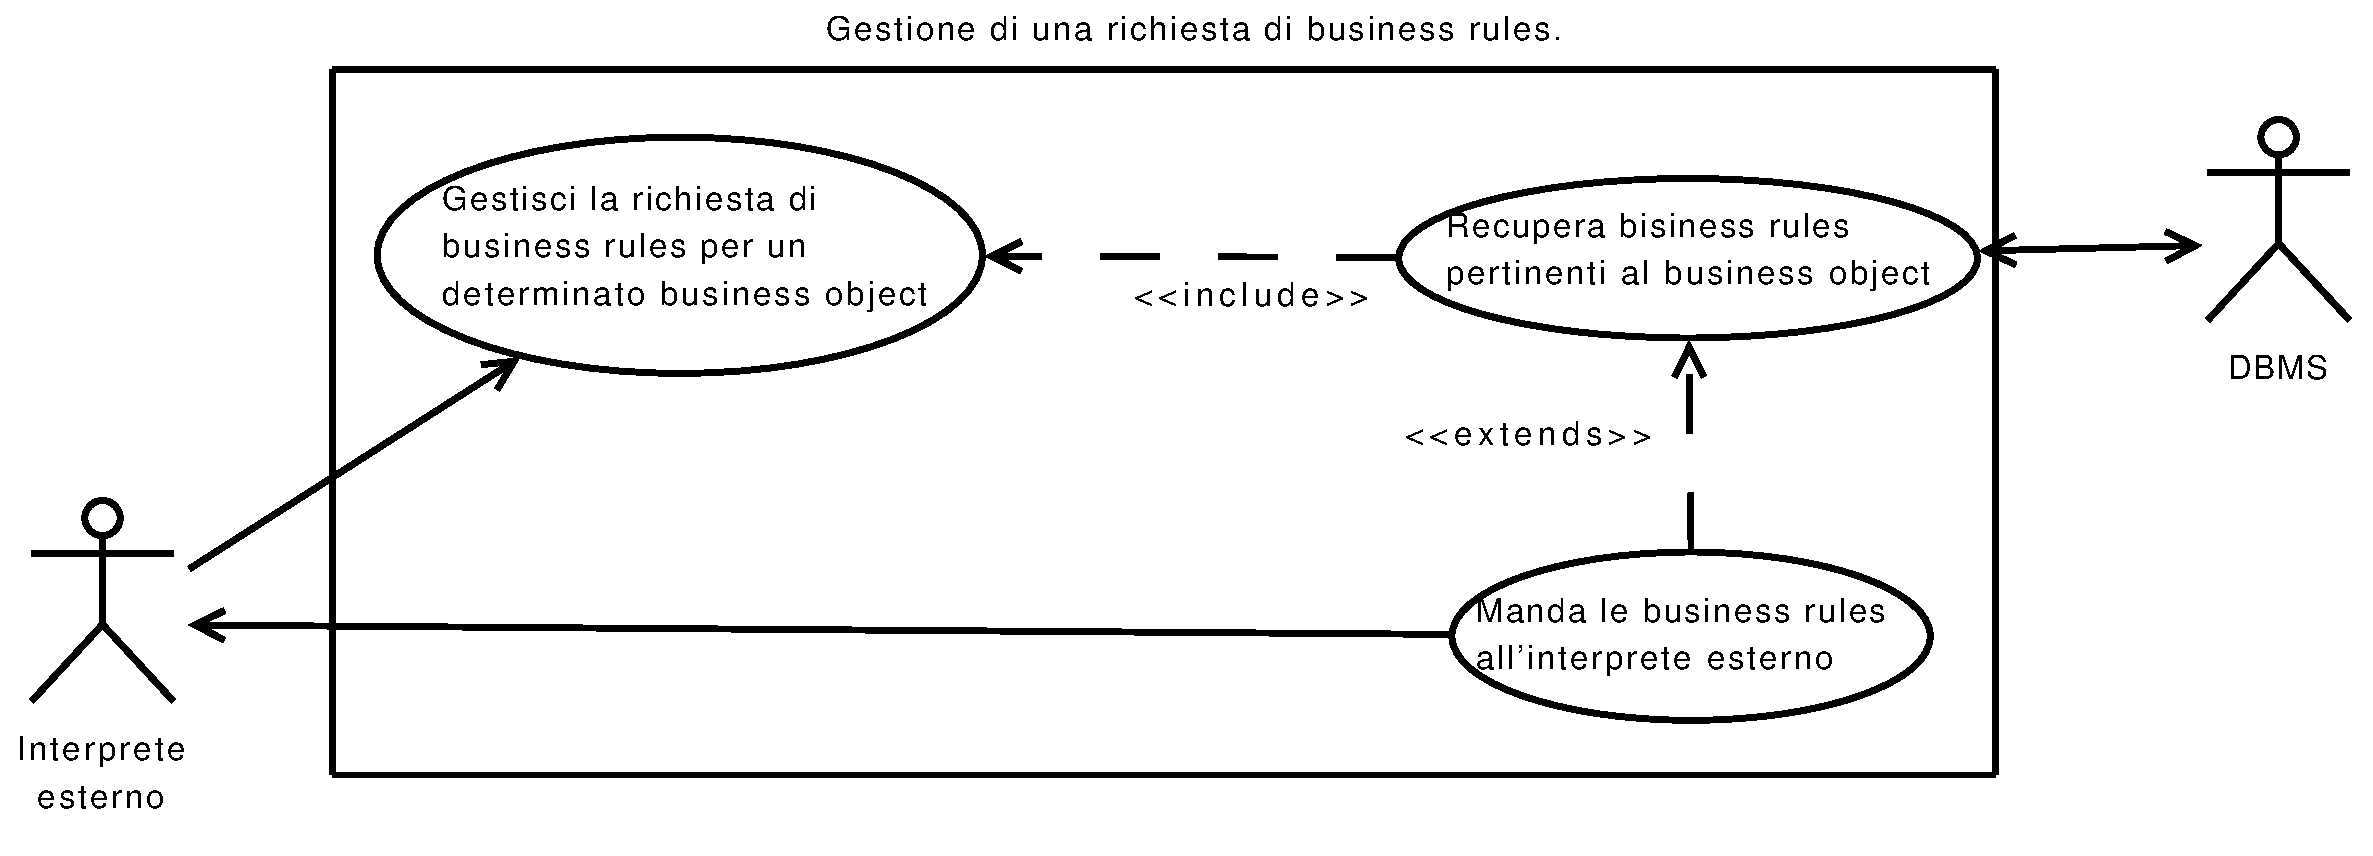
\includegraphics[width=1\textwidth]{use-case/Recupera-regole.eps}\
\end{center}

\subsection{Gestione della richiesta.}
\textbf{Attori coinvolti:} L'interprete esterno fornito dall'azienda che richiede la validazione di un business object.\\
\textbf{Scopo e descrizione sintetica:} Il sistema riceve una richiesta di validazione per un business object.\\
\textbf{Flusso di eventi:} Il sistema ha ricevuto la richiesta di validazione per un determinato business object.\\
\textbf{Precondizioni:} L'utente ha richiesto di validare un business object.\\
\textbf{Postcondizioni} Recupero delle regole pertinenti dal \underline{DBMS} .

\subsection{Recupera \\underline{Business Rules} pertinenti.}
\textbf{Attori coinvolti:} Il \underline{DBMS} che si occuper\`a di recuperare le regole\\
\textbf{Scopo e descrizione sintetica:} Il sistema chiede al \underline{DBMS} di recuperare le regole dal repository.\\
\textbf{Flusso di eventi:} Il sistema richiede al \underline{DBMS} di estrarre dal repository tutte le regole riguardanti quel business object.\\
\textbf{Precondizioni:} Il sistema ha acquisito la richiesta di validazione per un determinato business object.\\
\textbf{Postcondizioni} Il \underline{DBMS} riceve la richiesta di recuperare delle \\underline{Business Rules} dal repository.
\subsection{Manda le \\underline{Business Rules} all'interprete.}
\textbf{Attori coinvolti:} L'interprete esterno fornito dall'azienda che riceve le \\underline{Business Rules} per poter validare il suo business object.\\
\\textbf{Scopo e descrizione sintetica:} Il sistema ricevute le regole dal \underline{DBMS} le invia all'interprete esterno.\\
\textbf{Flusso di eventi:} Il sistema ricevute dal \underline{DBMS} tutte le regole riguardanti un determinato business object le invia all'interprete esterno.\\
\textbf{Precondizioni:} Il \underline{DBMS} ha terminato il recupero di tutte le \\underline{Business Rules} che riguardano il business object dato.\\
\textbf{Postcondizioni} L'interprete utilizzer\`a le \\underline{Business Rules} appena ricevute.

\section{Requisiti funzionali}
\begin{itemize}
\item[F1]{Si dovr\`a creare un linguaggio per la rappresentazione di \\underline{Business Rules}. [C04]}
\item[F2]{Il sistema dovr\`a fornire un validatore che consenta l'accettazione di nuove \\underline{Business Rules} soltanto se esse sono scritte secondo le specifiche del linguaggio creato. [C04]}
\item[F3]{Il sistema dov\`a inserire nel repository la nuova \underline{Business Rule} dopo la sua accettazione da parte del validatore. [C04]}
\item[F4]{Il sistema deve informare l'utente dell'esito della validazione di una nuova \underline{Business Rule}. Se la validazione \`e andata a buon fine l'utente deve essere informato in maniera chiara del buon esito e del tempo di risposta della validazione. Se la regola non viene accettata l'utente deve essere informato in maniera chiara di dove la sua regola non rispetta le specifiche del linguaggio. [C04]}
\item[F5]{Nell'interagire col repository il sistema dovr\'a appoggiarsi ad un \underline{DBMS} esterno. [I02]}
\item[F6]{Il sistema deve essere in grado di interfacciarsi con l'interprete esterno fornito dall'azienda proponente provvedendo ad esso le regole business da eseguire. [I02]}
\item[F7]{Il sistema dovr\`a consentire la cancellazione di \underline{Business Rules} all'interno del repository. [I02]}
\item[F8]{Il sistema dovr\`a essere dotato di un'interfaccia grafica minimale che consenta di definire una nuova \underline{Business Rules} e una volta validata inserirla nel repository. Tale interfaccia dovr\`a inoltre consentire di cancellare \underline{Business Rules} dal repository. Tutto ci\`o servir\`a a testare in modo rapido e chiaro il corretto funzionamento del prodotto. [I02]}
\item[F9]{ DEPRECATO : Il validatore deve essere dotato di un metodo per il controllo di coerenza tra \\underline{Business Rules}. Esso verificher\`a cio\`e se la \underline{Business Rule} da inserire nel repository entra in conflitto con le altre gi\`a presenti. Pi\`u dettagliatamente tale validatore dovr\`a verificare che le \\underline{Business Rules} presenti nel repository rappresentino un insieme soddisfacibile e non rigettino un qualunque insieme di valori possibili per i business objects. [C04]}
\item[F10]{Il validatore nel validare una \underline{Business Rule} deve poter accedere ai campi del business object ad essa associato, qualora la \underline{Business Rule} utilizzi tali campi. [I02]}
\item[F11]{Ad ogni business rule \`e associato un business object nel quale vanno eventualmente ricercati i campi dati utilizzati nella business rule. [I02]}
\end{itemize}

\section{Requisiti di usabilit\`a}
\begin{itemize}
\item[NU1]{Il linguaggio dovr\`a essere di alto livello. Dovr\`a cio\`e essere semplice da capire per un utente con bassa conoscenza informatica. [I01]}
\item[NU2]{Il linguaggio deve fornire funzioni primitive per le operazioni base tra i dati, come la somma, la media aritmetica e la negazione logica. [I01]}
\item[NU3]{Ad ognuno dei confronti presenti in una business rule deve essere possibile, da parte dell'utente, associare un messaggio che aiuti l'utente finale (ossia quello che chiede la validazione di un business object) a capire dove la validazione ha riscontrato problemi. [I02]}
\end{itemize}

\section{Requisiti di portabilit\`a}
\begin{itemize}
\item[NPo1]{Il formato di salvataggio delle business rules e del repository deve essere XML. [C04]}
\end{itemize}
\section{Requisiti prestazionali}
\begin{itemize}
 \item[NPr1]{Il \underline{DBMS} che andr\`a a interagire con il repository dovr\`a garantire una buona velocit\`a nell'interrogazione (mediante query) del file XML, anche in presenza di un consistente popolamento dello stesso. [I02]}
\item[NPr2]{Ad ogni business rule deve venire associata una stringa identificativa univoca per consentire un'efficiente indicizzazione delle business rules nel repository. [I02]}
\end{itemize}

\section{Requisiti di qualit\`a}
\begin{itemize}
\item[NQ1]{Il linguaggio dovr\`a permettere tutte le operazioni consentite tra scalari e matrici. Il validatore di conseguenza valider\`a solo le operazioni consentite. [I01]}
\item[NQ2]{Il progetto verr\`a accompagnato da un manuale che descriver\`a il linguaggio di definizione delle business rules. [C04]}
\item[NQ3]{Il progetto verr\`a accompagnato dalla descrizione delle API relative al validatore e al \underline{DBMS}. [C04]}
\end{itemize}
\newpage


\chapter{Appendice}
\section{Tracciamento relazione use case - requisiti}
\large{
\begin{tabular}{l}

\textbf{Inserimento e cancellazione di business rule dal repository}\\ \\

\begin{tabular}{||p{8cm}||p{4cm}||} \hline
\textbf{Use-case} & \textbf{Requisiti associati} \\ \hline
\textbf{Inserisci nuova business rule} & F2 - F8 - NU1 \\ \hline
\textbf{Valida business rule} & F2 - F3 - F4 - F5 - F8 - NPr1 - NQ1 \\ \hline
\textbf{Controlla la semantica} & F2 - F4 - F10 - NQ1\\ \hline
\textbf{Controlla sintassi} & F2 - F4 - NU2 - NQ1\\ \hline
\textbf{Richiedi al \underline{DBMS} di inserire nel repository} & F3 -  F5 -  NPo1 \\ \hline
\textbf{Restituisci messaggio di errore} & F2 - F4 - F10 - NU3 \\ \hline
\textbf{Richiedi al \underline{DBMS} di cancellare dal repositiry} & F7 - F8 \\ \hline
\end{tabular} \\ \\

\textbf {Gestione di una richiesta di business rule}\\ \\

\begin{tabular}{||p{8cm}||p{4cm}||} \hline
\textbf{Gestisci la richiesta di business rule per un determinato business object} & F6 - F10 - F11 \\ \hline
\textbf{Recupera business rule pertinenti al business object} & F5 - NPr1 - NPr2 \\ \hline
\textbf{Manda la business rule all'interprete esterno} & F6 \\ \hline
\end{tabular} \\
\end{tabular}
}

\section{Tracciamento relazione inversa: requisiti - use case}
\large{
\begin{tabular}{l}
\begin{tabular}{||p{2cm}||p{10cm}||} \hline
\textbf{Requisito} & \textbf{Use-case associato} \\ \hline
\textbf {F2} & \begin{itemize}
\item Inserisci nuova business rule
\item Valida busness rule
\item Controlla la semantica
\item Controlla sintassi
\item restituisci messaggio di errore
\end{itemize} \\ \hline
\textbf{F3} & \begin{itemize}
\item Valida business rule
\item Richiedi al \underline{DBMS} di inserire nel repository
\end{itemize} \\ \hline
\textbf{F4} & \begin{itemize}
\item Valida business rule
\item Controlla la semantica
\item Cotrolla sintassi
\item Restituisci messaggio di errore
\end{itemize} \\ \hline
\textbf{F5} & \begin{itemize}
\item Valida business rule
\item Richiedi al \underline{DBMS} di inserire nel repository
\item Recupera business rule pertinenti al business object
\end{itemize} \\ \hline
\textbf{F6} & \begin{itemize}
\item Gestisci la richiesta di business rule per un determinato business object
\item Manda la business rule all'interprete esterno
\end{itemize} \\ \hline
\end{tabular}
\end{tabular}

\begin{tabular}{l}
\begin{tabular}{||p{2cm}||p{10cm}||} \hline
\textbf{F7} & \begin{itemize}
\item Richiedi al \underline{DBMS} di cancellare dal repository
\end{itemize}\\ \hline


\textbf{F8} & \begin{itemize}
\item Inserisci nuova business rule
\item Valida business rule
\item Richiedi al \underline{DBMS} di cancellare dal repository
\end{itemize} \\ \hline
\textbf{F10} & \begin{itemize}
\item Controlla la semantica
\item Restituisci messaggio di errore
\item Gestisci la richiesta di business rule per un determinato business object
\end{itemize} \\ \hline
\textbf{F11} & \begin{itemize}
\item Gestisci la richiesta di business rule per un determinato business object
\end{itemize} \\ \hline
\textbf{NU1} & \begin{itemize}
\item Inserisci nuova business rule
\end{itemize} \\ \hline
\textbf{NU2} & \begin{itemize}
\item Controlla sintassi
\end{itemize} \\ \hline
\textbf{NU3} & \begin{itemize}
\item Restituisci messaggio di errore
\end{itemize} \\ \hline
\textbf{NPo1} & \begin{itemize}
\item Richiedi al \underline{DBMS} di inserire nel repository
\end{itemize} \\ \hline
\textbf{NPr1} & \begin{itemize}
\item Valida business rule
\item Recupera business rule pertinenti al business object
\end{itemize} \\ \hline

\end{tabular}
\end{tabular}

\begin{tabular}{l}
\begin{tabular}{||p{2cm}||p{10cm}||} \hline


\textbf{NPr2} & \begin{itemize}
\item Recupera business rule pertinenti al business object
\end{itemize} \\ \hline

\textbf{NQ1} & \begin{itemize}
\item Valida business rule
\item Controlla la semantica
\item Controlla sintassi
\end{itemize} \\ \hline
\end{tabular} \\
\end{tabular}
}

\end{document}
